\documentclass[11pt]{article}

\usepackage{amsmath}
\usepackage{textcomp}
\usepackage[top=0.8in, bottom=0.8in, left=0.8in, right=0.8in]{geometry}
% Add other packages here %
\usepackage{amssymb}
\usepackage{mathtools}
\usepackage{graphicx}
\usepackage{subcaption}
\usepackage[export]{adjustbox}
\usepackage{multirow}
\newcommand{\N}{\mathbb{N}}

% Put your group number and names in the author field %
\title{\bf Excercise 3\\ Implementing a deliberative Agent}
\author{Group \textnumero$75$: Thomas KIMBLE, Jules AFRESNE}

% N.B.: The report should not be longer than 3 pages %

\begin{document}
\maketitle

\section{Model Description}

\subsection{Intermediate States}
% Describe the state representation %
Each State is represented by the following characteristics:
\begin{itemize}
    \item \textit{currentCity:} This is the city where the agent is currently found.
    \item \textit{actionList:} This is a list of the actions previously taken to get to this state. Each action is added to this list to allow cost calculations and plan execution once a goal state is reached.
    \item \textit{availableTasks:} This is a TaskSet containing the available tasks in a simulation. The agent has not picked up any of these tasks, they will have to be picked up and delivered.
    \item \textit{transportedTasks:} This is a TaskSet containing the tasks to be delivered by the agent. These tasks have already been picked up and are waiting to be delivered.
    \item \textit{currentWeightVehicle:} This is the weight that a vehicle is currently carrying. Thanks to it the free weight left in the vehicle can be computed.
    \item \textit{gCost, hCost, fCost:} gCost is the cost function of the actions that lead up to the current state. For fCost and hCost see part 2.3 Heuristic Function.
    \item \textit{isGoal:} This is a boolean that is false if we are in an intermediate state, and true if in a goal state.
\end{itemize}

\subsection{Goal State}
% Describe the goal state %
\indent \indent We are in a goal state once all tasks have been picked up and delivered. In our model this is the case when \textit{availableTasks} and \textit{transportedTasks} are both empty. If only \textit{availableTasks} is empty we could still have tasks being transported, so we need to assure that \textit{transportedTasks} is also empty. In this case the boolean \textit{isGoal} is true.

\subsection{Actions}
% Describe the possible actions/transitions in your model %
\indent \indent We want to create a tree with the next possible states after the current one, and so on to figure out a plan. Therefore, from the current state we create a list of "children" states obtained by two possible actions: \textit{Pick Up} and \textit{Delivery}. The number of possible actions, and therefore the number of child states, is equal to the number of tasks being transported and remaining. Each possible action to get to a future state is added to the \textit{actionList} of the said future state.

For the \textit{Pick Up} action we scroll through the \textit{availableTasks} TaskSet of the current state and first check if the task is too heavy. If so we do not proceed with this action. If not we proceed by picking up the task or by going to a new city and picking it up. The vehicle weight is updated, we remove the new task from the \textit{availableTasks} of the next state and add the new task to the \textit{transportedTasks} of the next state.

For the \textit{Delivery} action we scroll through the \textit{transportedTasks} TaskSet of the current state and deliver a carried task to the current city or a new city. The vehicle weight is updated and we remove the new task from the \textit{transportedTasks} TaskSet of the next state.


\section{Implementation}

\subsection{BFS}
% Details of the BFS implementation %
\indent \indent First of all we create an initial state with all of the vehicle parameters and available tasks, given it an initial $gCost$ of zero. We declare four State Array Lists: an open list $Q$, the next layers open list $nextLayerQ$, a closed list $C$ and a goal states list $goalState$. We implement the Breadth First Algorithm filling up these lists to find our Goal States in an optimal way. We sorted the $nextLayerQ$ list in order of increasing $gCost$ to optimise the algorithm.

To find the optimal solution, we compare the costs of all of the goal states and select the state with the minimal cost. This step requires more time and computational power, but it assures that the optimal solution is returned rather than the first found solution.

\subsection{A*}
% Details of the A* implementation %
\indent \indent As in the BFS algorithm we first create an initial state with all of the vehicle parameters and available tasks, given it an initial $gCost$ of zero. We declare two State Array Lists: and open list $Q$ and a closed list $C$. We implement the A* algorithm with the heuristic function described in part 2.3 to assure that the optimal solution is found. We sorted the $Q$ list in order of increasing $fCost$ to optimise the algorithm.

\subsection{Heuristic Function}
% Details of the heuristic functions: main idea, optimality, admissibility %
\indent \indent The heuristic function $h(n)$ corresponds to the estimated minimum cost to get from the current state to a goal state. Let us consider our model where we have three possible cases:

\begin{itemize}
    \item One single possible action, $a_1$ = pick up a task. Here the goal state is the state after the next one. Therefore the heuristic function is equal to: 
        \begin{equation}
            h(n) = (distanceToTask + distanceToDelivery)*costPerKm = h^*(n)
        \end{equation}
    \item One single possible action, $a_2$ = deliver a task. Here the next state is a goal state. Therefore the heuristic function is equal to: 
        \begin{equation}
            h(n) = distanceToDelivery*costPerKm = h^*(n)
        \end{equation}
    \item k possible actions, $a_1, a_2, ..., a_k$, $k\in \N$ (pick up and/or delivery). Here the heuristic function: 
        \begin{equation}
            h(n) = max(h(a_i)) \leq h^*(n), \: \: \: \: \: i= 1, ... \:, k
        \end{equation}
\end{itemize}

In all three of these cases we assure that $h(n)$ under-estimates the true cost, but we try to get $h(n)$ as close as $h^*(n)$ to reduce the necessary number of iteration to find a goal state. This confirms that A* will always find the optimal solution.

\section{Results}

\subsection{Experiment 1: BFS and A* Comparison}
% Compare the two algorithms in terms of: optimality, efficiency, limitations %
% Report the number of tasks for which you can build a plan in less than one minute %

\subsubsection{Setting}
% Describe the settings of your experiment: topology, task configuration, etc. %
For Table 1 we observe a single deliberative agent using the BFS and A* algorithms in the \textbf{France topology} with four to eleven tasks. Each vehicle has a speed of 220, with a capacity of 30.

\subsubsection{Observations}
% Describe the experimental results and the conclusions you inferred from these results %

\indent \indent Table 1 shows us that for both algorithms the number of iterations and the execution time grow exponentially with each added task. However the A* algorithm is much faster and can perform with more tasks than the BFS. We also notice that the plan cost for each of the different number of tasks is the same for both algorithms. These observations confirm that A* is faster and uses less resources than BFS, however in both cases we find the optimal solution.

\begin{table}[ht]
\centering
\begin{tabular}{|c|l||c|c|c|c|c|c|c|c|}
\hline
\multicolumn{2}{|c||}{Number of Tasks} & 4 & 5 & 6 & 7 & 8 & 9 & 10  &  11\\ \hline \hline
\multirow{3}{*}{BFS}  & Iterations & 490 & 2340 & 9997 & 37 808 & 141948 & - & - & - \\ \cline{2-10} 
                   & Time [s] & 0.017 & 0.038 & 0.399 & 3.355 & 48.317 & - & - & - \\ \cline{2-10} 
                   & Cost & 15 495 & 15 495 & 21 405 & 21 405 & 21 405 & - & - & - \\ \hline \hline
\multirow{3}{*}{A*}  & Iterations & 44 & 103 & 478 & 973 & 3 132 & 27 636 & 43 861 & 138 662 \\ \cline{2-10} 
                   & Time [s] & 0.007 & 0.012 & 0.035 & 0.057 & 0.192 & 7.75 & 23.548 & 286.713 \\ \cline{2-10} 
                   & Cost & 15 495 & 15 495 & 21 405 & 21 405 & 21 405 & 23 955 & 23 955 & 23 955 \\ \hline
\end{tabular}
\label{tab:1}\caption{Performance comparison between BFS and A* (number of iterations, execution time and cost)}
\end{table}

\subsection{Experiment 2: Multi-agent Experiments}
% Observations in multi-agent experiments %

\subsubsection{Setting}
% Describe the settings of your experiment: topology, task configuration, etc. %

We observe 1, 2 and 3 deliberative agents using the A* in the \textbf{Switzerland topology} with 9 tasks. Each vehicle has a speed of 90, with a capacity of 30. We plot the Reward per km as a function of time.

\subsubsection{Observations}
% Describe the experimental results and the conclusions you inferred from these results %
\indent \indent If the current plan is no longer possible, we calculate a new plan and we notice that each new calculated plan is obtained faster because there will be less tasks available. We also notice that the more agents there are, the faster the tasks are completed, indeed $t_a = 14.8s$, $t_b = 10.8s$ and $t_c = 9.3s$. Nevertheless agents may lose their efficiency because each one computes its own plan without considering the other's plan. This depends a lot about the configuration especially the number of tasks to deliver and the initial position of vehicles. We calculate the average reward per second : $R_a^{avg} = 0.18$ per $s$, $R_b^{avg} = 0.19$ per $s$ and $R_c^{avg} = 0.16$ per $s$. In our case, the model where there are two agents is the most effective.

\begin{figure}[ht]
\centering
  \begin{subfigure}[t]{0.175\textwidth}
    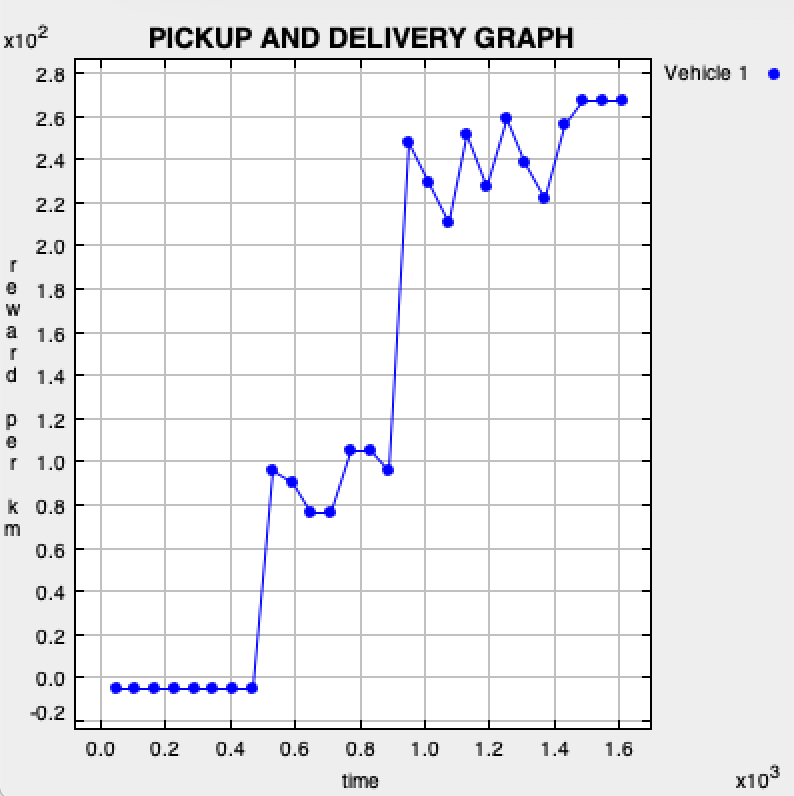
\includegraphics[width=\textwidth, frame]{9T1A.png}
    \caption{Single agent}
    \label{fig:2a}
  \end{subfigure}
  %
  \begin{subfigure}[t]{0.175\textwidth}
    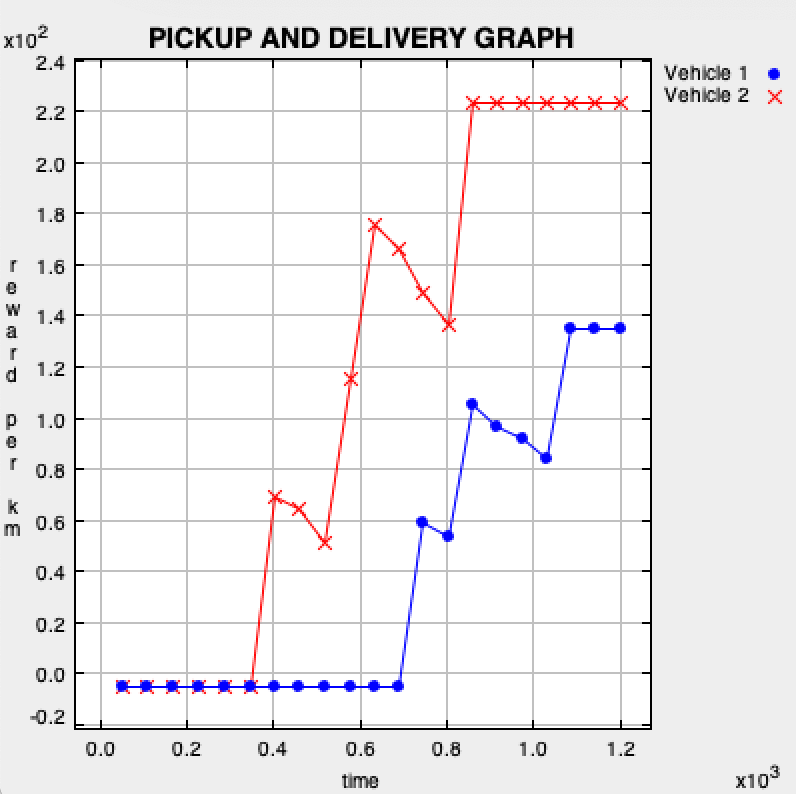
\includegraphics[width=\textwidth, frame]{9T2A.png}
    \caption{Two agents}
    \label{fig:2b}
  \end{subfigure}
  %
  \begin{subfigure}[t]{0.175\textwidth}
    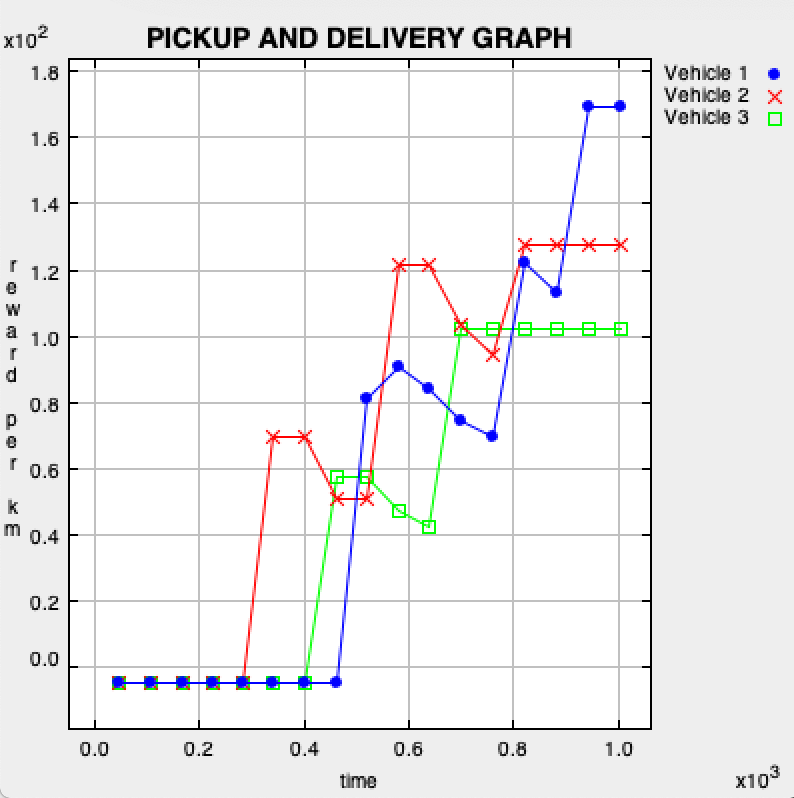
\includegraphics[width=\textwidth, frame]{9T3A.png}
    \caption{Three agents}
    \label{fig:2c}
  \end{subfigure}
\end{figure}

\end{document}